\section{Representations}\label{sec:representations}
Due to the flexibility of networks, different representations of the connectomes can be studied, which we organize into four categories. In the following sections, we first formally define a network and then describe the four different frameworks of studying connectomics data. All frameworks provide complementary insights and understanding of the connectomes. 

\subsection{Graph/Network}
\label{sec:unwt_graph}
A graph, or network, $\mathcal{G}$, is defined as an ordered set of vertices and edges $(V, E)$ where $V$ is the vertex set, and $E$, the set of edges, is a subset of the Cartesian product of $V \times V$. That is, a graph has at most a single edge for each pair of unique vertices. A vertex set is represented as $V=\{1, 2, \ldots, n\}$ where $|V| = n$, and an edge exists between vertices $i$ and $j$ if $(i, j)\in E$. An unweighted graph is a graph in which we are only concerned with the presence (or absence) of an edge. Each graph has an associated adjacency matrix $\A \in \left\{0, 1\right\}^{n\times n}$ where $\A_{ij}$ represents the presence (or absence) of the edge between nodes $i$ and $j$. Note that $\A$ provides a unique representation of $\mathcal{G}$; that is, there exists a $1$-to-$1$ relationship between a graph and its adjacency matrix. 

The above definition can be further extended in two ways: 
\begin{enumerate}
    \item Weighted graphs - the edges can take on arbitrary values, typically a real number. For example, the edge weight in human structural connectomes are non-negative integers that represent the number of estimated neuronal fibers that traverse from one region of the brain to another. Thus, each weighted graph has an adjacency matrix $\A\in\RR^{n \times n}$ where $\A_{ij}$ represents the edge weight.
    \item Directed graphs - $E$ is now an \textit{ordered} set of edges. Each edge has an associated direction, and a directed edge exists between vertices $i$ and $j$ if $(i,j)\in E$. In undirected graphs, the associated adjacency matrix $\A$ is symmetric, but in directed graphs, $\A$ is not necessarily symmetric, that is, it is possible that $\A_{ij}\neq\A_{ji}$, for any $i, j\in V$.
\end{enumerate}

For the remainder of the paper, graphs are considered undirected and unweighted and with no self-loops, that is $\text{diag}(\A) = \Vec{0}$, unless specified otherwise.

\subsection{Bag of Features}\label{sec:bag-of-features}
Network statistics, or features, are abstract representations that capture either global or local structures of a network \cite{priebe_coppersmith_rukhin_2010,mhembere2013computing}. This method computes a set of network statistics for each network, and analyzes differences between, or among, populations. For example, when comparing populations of networks from healthy and individuals with depression, the difference in global clustering coefficient, which measures how likely vertices tend to cluster together, can be computed \cite{Bullmore2009-yj}. These network statistics have enjoyed applications in many connectomics studies that compare different populations of networks \cite{bullmore2011brain, ghoshdastidar2017two}. However, there are infinitely number of such statistics, and we lack general guidance in which statistics to compute. Furthermore, no set of network statistics can adequately characterize a network \cite{chen2018same,matejka2017same}. These considerable shortcomings further motivates the use of other representations of networks, and below examples demonstrate the shortcomings of studying bags of features.

\subsubsection{Non-identifiability of graph features}
Summary statistics, such as the mean, variance, and correlation, are often used to describe real valued datasets, which can be insightful in understanding the data. However, the Anscombe's quartet illustrates four drastically different distributions of eleven points that have the same summary statistics \cite{anscombe1973graphs}. This suggest that any small number of summary statistics can fail to meaningfully characterize the data. 

In network analysis, variety of network level statistics can be computed to summarize networks. Similar to the Anscombe's quartet, networks with different topologies can have the same network features as shown in Figure \ref{fig:exp5}. These four networks have the same number of vertices, edges, triangles, and global clustering coefficient, but have different properties such as connectedness and symmetry. Other works have also explored the distributions of network statistics \cite{chen2018same,matejka2017same}. 

\begin{figure}
    \centering
    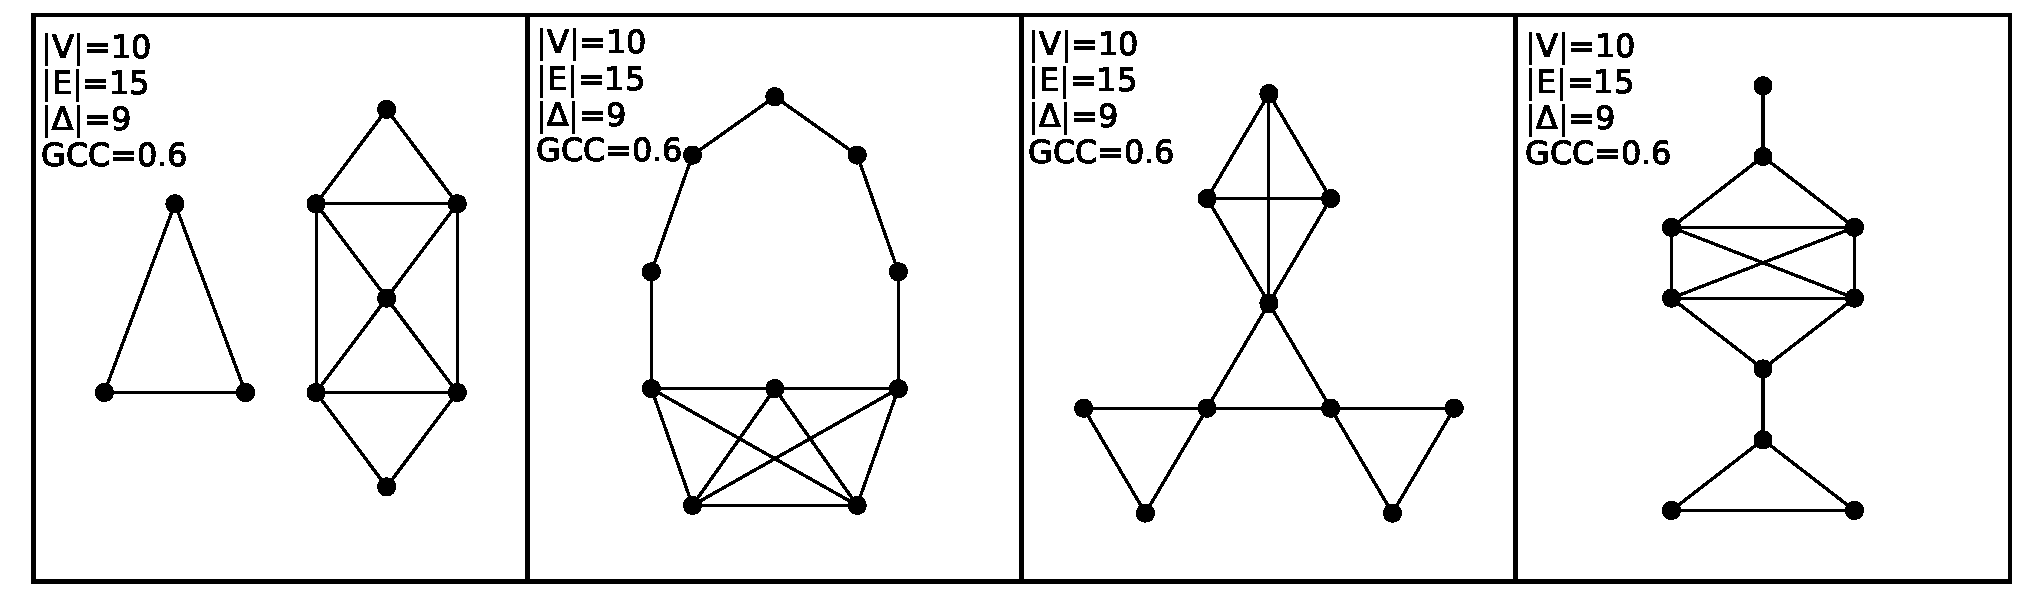
\includegraphics[width=.9\textwidth]{figures/dnd/exp5_10nodes_row}
    \caption
    [Four Networks with Same Network Statistics.]
    {\textbf{Four Networks with Same Network Statistics.} Each network has 10 vertices ($\abs{V}$), 15 edges ($\abs{E}$), 9 triangles ($\abs{\Delta}$), and the global clustering coefficient (GCC) is 0.6. However these graphs have distinctive topologies. For example, the left-most network is disconnected, while others are connected. This suggest that given a small set of network statistics, one cannot identify from which network the features are computed.
    }
    \label{fig:exp5}
\end{figure}

\subsubsection{Network features are correlated and relatively uninformative}
We consider all non-isomorphic, undirected, binary networks with 10 vertices, which results in $\approx12$ million networks. Formally, $\mathcal{G}$ and $\mathcal{H}$ are isomorphic networks when there exists a vertex permutation function $f:V(\mathcal{G})\rightarrow V(\mathcal{H})$ such that if edge $(u,v)\in E(\mathcal{G})$, then $(f(u), f(v))\in E(\mathcal{H})$. Only non-isomorphic networks are considered since isomorphic networks have identical network features.

For each network, the following six graph network statistics are computed: 1) average path length (APL), 2) global clustering coefficient (GCC), 3) average clustering coefficient (ACC), 4) global efficiency (GE), 5) local efficiency (LE), and 6) modularity. These statistics are some of the most commonly computed statistics \cite{sporns2005human,Bullmore2009-yj}. The distribution of network statistics are plotted against modularity. 
The top row of Figure \ref{fig:exp6} shows that all of the network features are highly correlated with modularity.
We then constrain the networks in two different ways. First, we consider all networks with $20 \pm 2$ edges. Second, we choose a ``base'' network at random with 20 edges, and then identify all networks with no more than 3 edges different from the  base network. The distribution of each of the above network statistics on this subset of networks are computed for both constraints. The middle and bottom rows of Figure \ref{fig:exp6} show that constraining the networks in these ways hardly constrains the network features at all. Similar pattern is shown in the analysis of HCP data as shown in Supplemental Appendix \ref{sec:bag-of-features-hcp}. Changing only a few edges on a network can yield a network with almost any possible configuration according to these statistics, and therefore are inadequate to characterize these populations. Thus, when any given metric is correlated with a covariate of interest, so are many other metrics. Thus, claiming that a particular property of the brain ``explains'' a given phenotypic property of a person is spurious reasoning.

\begin{figure} 
    \centering
    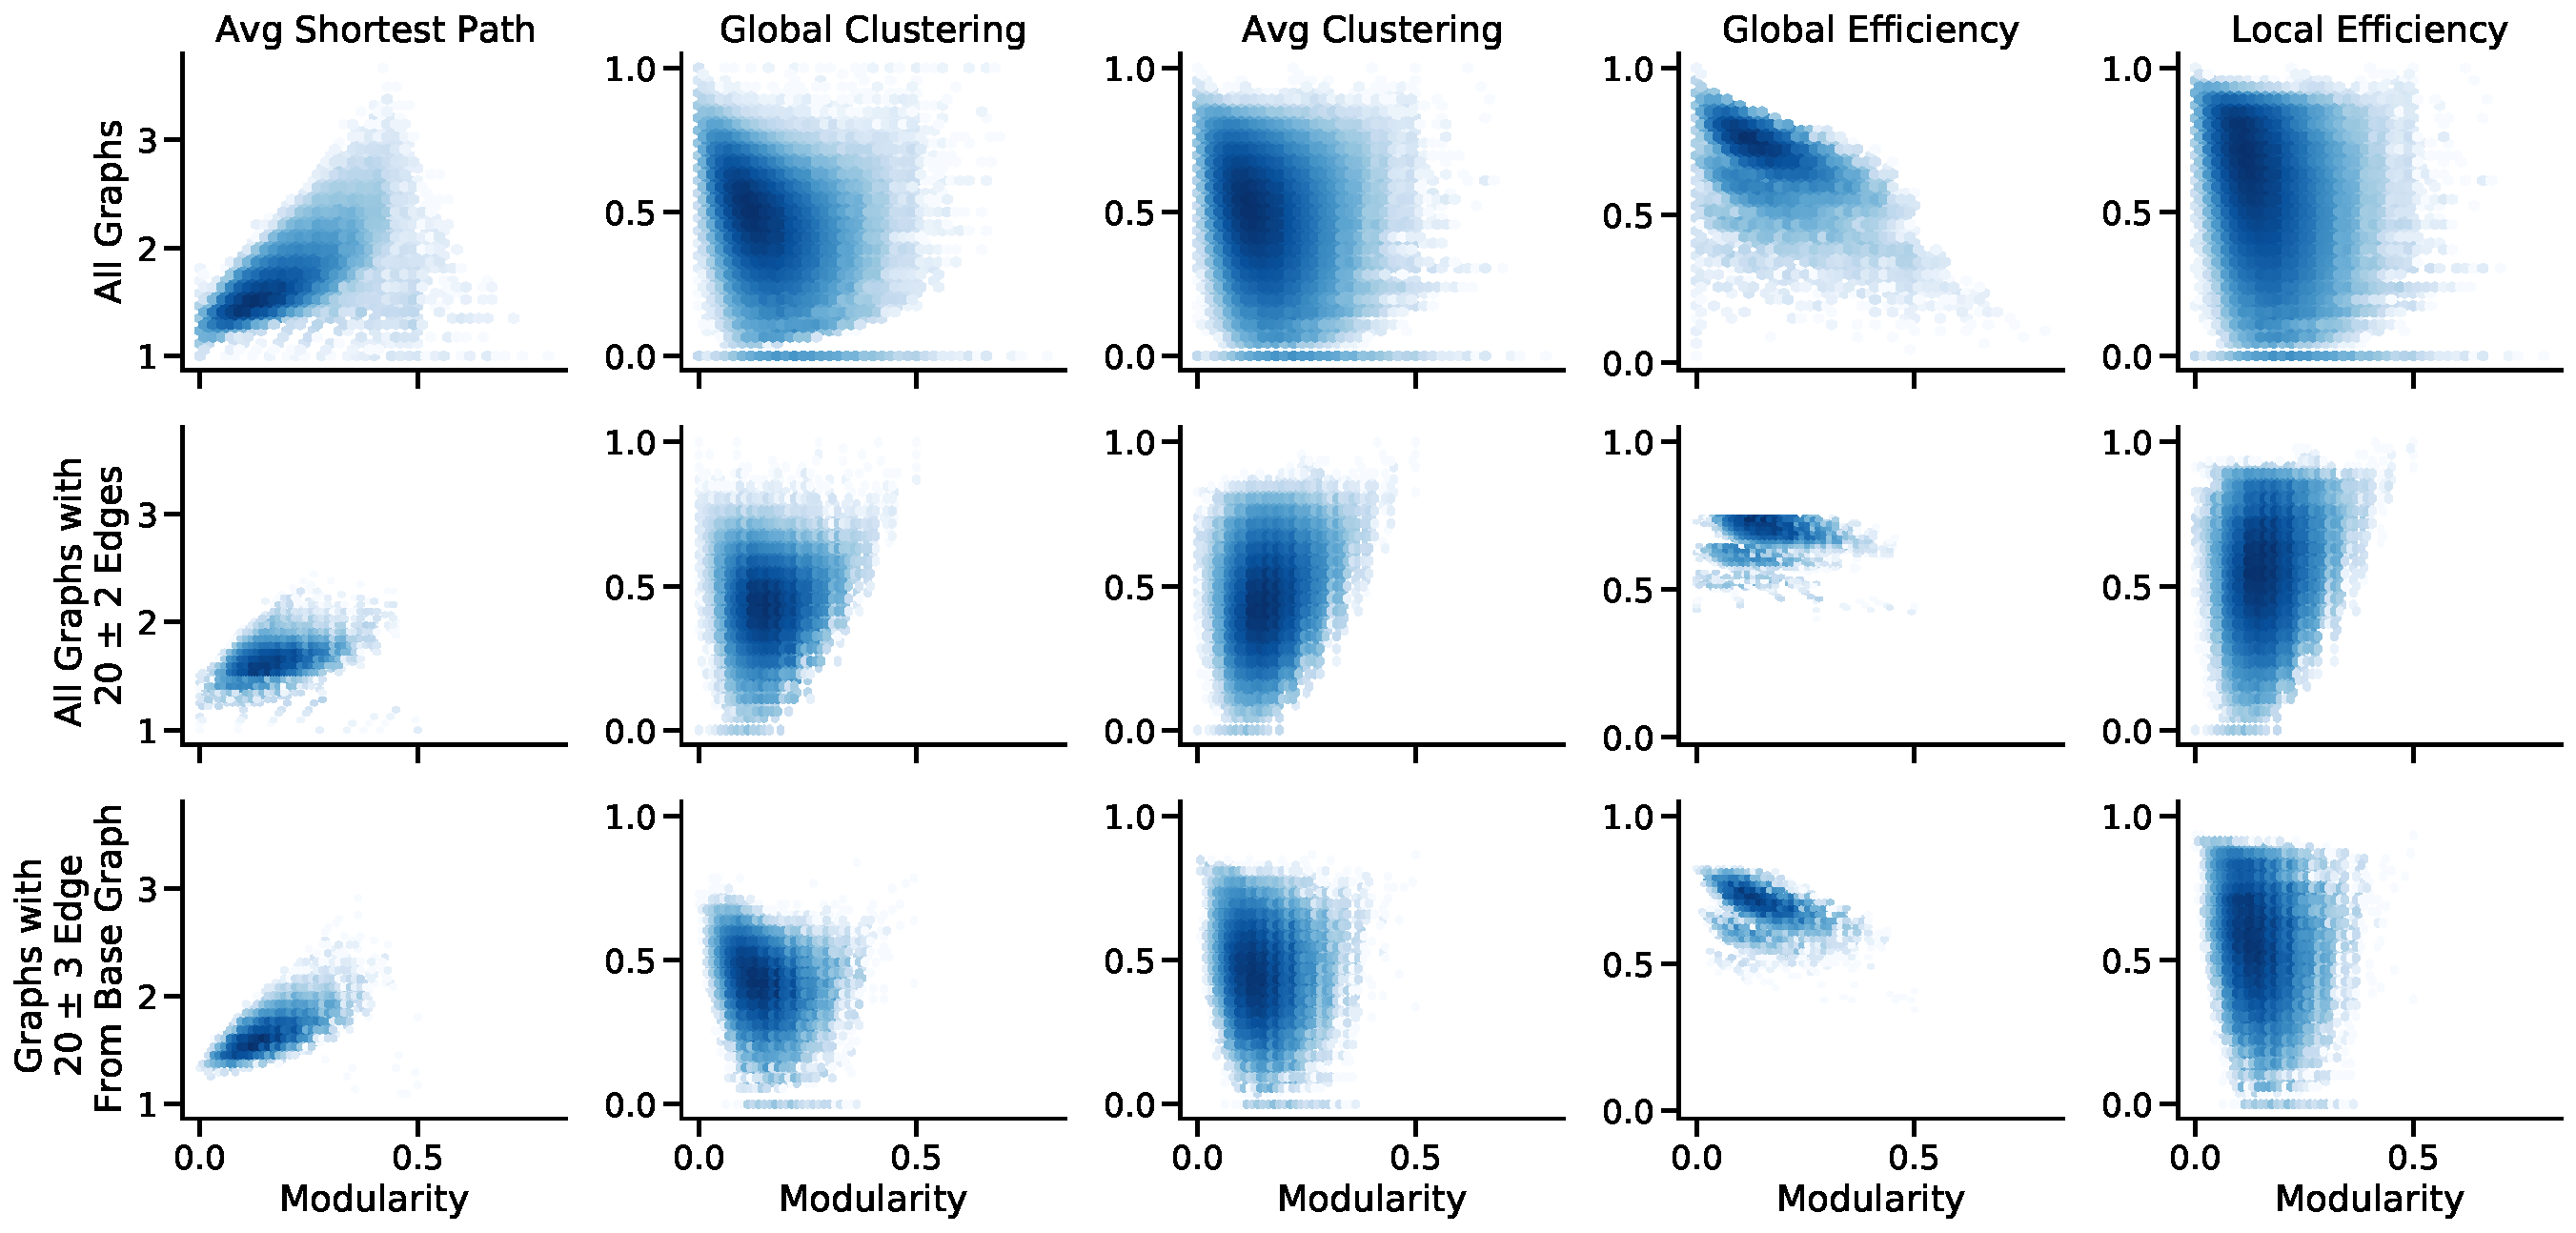
\includegraphics[width=\textwidth]{figures/dnd/density_num_edge_20_row}
    \caption
    [Density plots of network statistics.]
    {\textbf{Density plots of network statistics.} \textit{(Top Row)} The distributions of networks statistics for all possible 10-node networks are shown. \textit{(Middle Row)} Networks are constrained by only considering all networks with $20 \pm 2$ edges. \textit{(Bottom Row)} A base graph with $20$ edges is chosen at random, and only networks that have differences up to $3$ edges are considered. In both constrained set of networks, the distribution of these network statistics remains essentially unchanged. In other words, changing only a few edges on a network can yield a network with almost any possible configuration according to these statistics. }
    \label{fig:exp6}
\end{figure}

\subsection{Bag of Edges}\label{sec:bag_of_edges}
In this approach, the edges of connectomes are studied. Most commonly, each edge is studied independently, while ignoring any interactions between edges \cite{Craddock2013-qs,Varoquaux2013-hy,zhang2018mapping}. Univariate edge-wise testing can reveal easily interpretable relationships between specific edges and covariates through hypothesis testing. However, edge-wise testing requires performing multiple hypothesis tests, and multiple comparisons must be corrected to control the false positive rate \cite{Genovese2002-yq,Efron2008-zq}. While certain methods, such as Benjamini–Hochberg corrections, have strong theoretical guarantees, they require assumptions about the data, such as independence, that connectomics data do not satisfy \cite{Zalesky2010-ox,Benjamini1995-ij,Simes1986-gn}. On the other hand, Bonferroni corrections are considered too conservative, and, therefore, lack the sensitivity for connectomics \cite{Simes1986-gn}.

More intricate methods represent each connectome as a long vector containing all of its edges \cite{richiardi2011decoding, amico2017mapping}. Vector representations can allow for correlation of edges and direct application of common machine learning algorithms, but still discards the structural information in networks.

\subsection{Bag of Vertices}\label{sec:bag_of_nodes}
In this approach, the vertices of connectomes are analyzed while leveraging structural information, typically global structures, of the graphs. 
A common approach embeds the connectomes to learn a low-dimensional and Euclidean representation of the vertices \cite{grover2016node2vec, athreya2017statistical, arroyo2019inference}. Algorithms that operate on Euclidean data (e.g. Gaussian Mixture Model ($\gmm$) for clustering vertices, random forests for classifying vertices, multivariate hypothesis tests for testing for differences between vertices) can be employed for subsequent analysis \cite{priebe2017semiparametric, tang2018connectome}. 

\subsection{Bag of Communities}
Networks often contain structural information such as communities, which are subsets of vertices that behave similarly. For example, similar vertices can be defined by those that are more likely to be connected with each other than to other vertices.
The set of communities that comprise a network, called community structure, can describe both the local and global patterns of the network. At local-scale, we can examine the properties of vertices that are within the same community. At global-scale, we can measure associations between connectivity patterns of communities across groups or other covariates \cite{faskowitz2018weighted, kim2019graph, arroyo2020simultaneous}. Furthermore, the community structure in spatial resolution connectomes from human MRI can be used to delineate regions of the brain, called parcellations \cite{thirion2014fmri}.

Community detection in networks have been studied extensively \cite{newman2013spectral, fortunato2016community}. Typically, the community structure is identified by modularity optimization methods \cite{clauset2004finding, blondel2008fast}. In this paper, we present spectral methods that rely on statistical models for community detection, which have strong statistical guarantees for recovering true communities \cite{sussman2012consistent, lyzinski2016community, athreya2017statistical, arroyo2019inference}.
It is important to note that analysis of communities depends on the performance of the community detection algorithms.

\subsection{Bag of Networks}
In this approach, one or more groups of networks are studied in various settings, such as one- and two-sample hypothesis testing, and classification, using some representation of networks. For example, bag of vertices representation can be used to test whether two networks are different \cite{tang2017nonparametric, tang2017semiparametric}. For studying more than two networks, geometry in the space of the networks is defined and are represented in that geometry, which are then used for finding differences across groups \cite{ginestet2017hypothesis, xia2019matrix, arroyo2019inference}.

Another group of methods finds subsets of vertices, or a subgraph, that contain the most information about certain covariates \cite{vogelstein2012graph, wang2018signal,  relion2019network, wang2019symmetric, guha2020bayesian}. Estimating signal subgraphs is useful since networks can be extremely large (i.e. millions of vertices), which present computational challenges, and can potentially improve the performance of subsequent inference tasks, such as classification. 
Different approaches for finding the subgraph have been proposed, but all approaches leverage the network topologies inherent in connectomics data. 
